\documentclass{standalone}
\usepackage{tikz}
\usetikzlibrary{arrows,positioning,decorations.pathreplacing} 
\tikzset{
    %Define standard arrow tip
    >=stealth',
    %Define style for boxes
    point/.style={
           rectangle,
           rounded corners,
           draw=black, very thick,
           text width=6em,
           minimum height=2em,
           font=\sffamily,
           text centered},
    annote/.style={
          font=\sffamily
    },
    % Define arrow style
    arrow/.style={
           ->,
           thick,
           shorten <=2pt,
           shorten >=2pt,},   
}
\begin{document}
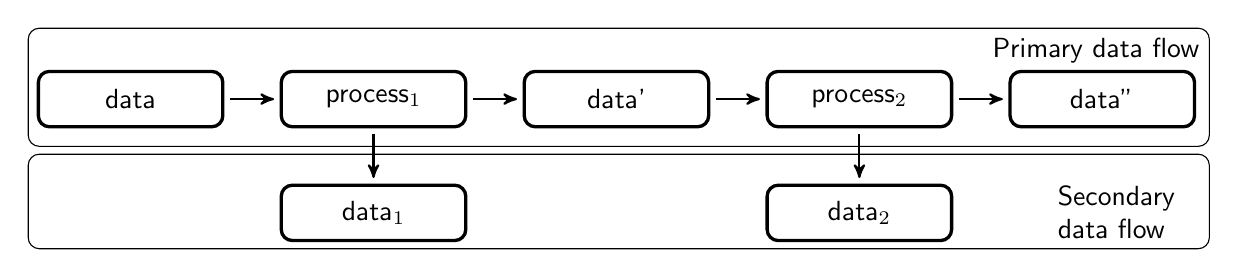
\begin{tikzpicture}
  \node[point] (in) {data};
  \node[point, right=7mm of in]  (mod1) {process$_1$};
  \node[point, right=7mm of mod1] (out1){data'};
  \node[point, right=7mm of out1] (mod2){process$_2$};
  \node[point, right=7mm of mod2] (out2){data''};
%  \node[point, above=7mm of mod1] (par1) {parameters$_1$};
% \node[point, above=7mm of mod2] (par2) {parameters$_2$};
  \node[point, below=7mm of mod1] (log1){data$_1$};
  \node[point, below=7mm of mod2] (log2){data$_2$};
%\draw [rounded corners] (-1.3,1.0) rectangle ++(15.0,0.9) 
%      node [anchor=north east] {\textsf{End user}};

\draw [rounded corners] (-1.3,-0.6) rectangle ++(15.0,1.5) 
      node [anchor=north east] {\textsf{Primary data flow}};

\draw [rounded corners] (-1.3,-0.7) rectangle ++(15.0,-1.2) 
      node [anchor=south east, text width=18mm] {\textsf{Secondary data flow}};
  \path (in.east) edge[arrow] (mod1.west);
  \path (mod1.east) edge[arrow] (out1.west);
  \path (out1.east) edge[arrow] (mod2.west);
  \path (mod2.east) edge[arrow] (out2.west);
%  \path (par1.south) edge[arrow] (mod1.north);
%  \path (par2.south) edge[arrow] (mod2.north);
  \path (mod1.south) edge[arrow] (log1.north);
  \path (mod2.south) edge[arrow] (log2.north);
\end{tikzpicture}
\end{document}
